\documentclass[tikz,border=8pt]{standalone}
% Shared look for every TikZ diagram. Load with \input{../../tools/tikz-style.tex}
\usepackage[T1]{fontenc}
\usepackage{lmodern}
\renewcommand{\sfdefault}{lmr}  % diagrams use the same serif as the text
\usetikzlibrary{arrows.meta, positioning, shapes.geometric, calc, fit, backgrounds}
\definecolor{cblue}{HTML}{4C78A8}
\definecolor{corange}{HTML}{F58518}
\definecolor{cgreen}{HTML}{54A24B}
\definecolor{cred}{HTML}{E45756}
\definecolor{cpurple}{HTML}{B279A2}
\definecolor{cgrey}{HTML}{6B6B6B}
\tikzset{
  every picture/.style={font=\sffamily, line width=1.2pt},
  box/.style={draw=#1, fill=#1!12, rounded corners=4pt, align=center, inner sep=7pt, minimum height=1.1cm},
  box/.default=cgrey,
  arrow/.style={-{Stealth[length=3mm]}, draw=cgrey, line width=1.4pt},
  title/.style={font=\sffamily\bfseries\Large},
  note/.style={font=\sffamily\small, text=cgrey, align=center},
}
\AtBeginDocument{\hyphenpenalty=10000 \exhyphenpenalty=10000}

\begin{document}
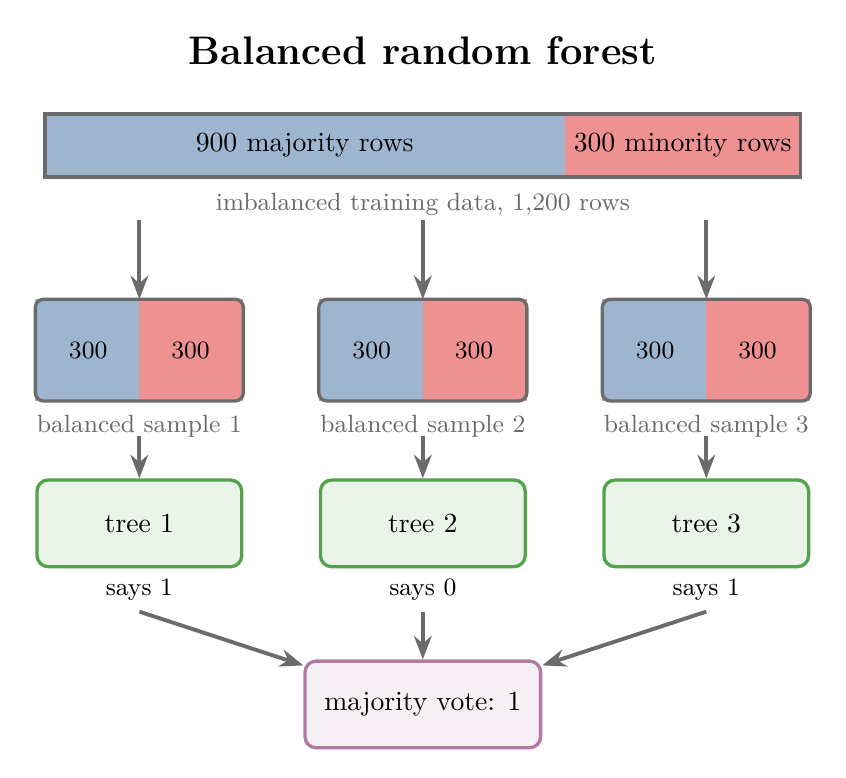
\begin{tikzpicture}[smp/.style={draw=cgrey, rounded corners=3pt, minimum width=2.6cm, minimum height=1.25cm, inner sep=0pt},
  tree/.style={box=cgreen, minimum width=2.6cm}]
  % the imbalanced training data: 900 majority (blue), 300 minority (red)
  \node[title] at (4.2,2.4) {Balanced random forest};
  \fill[cblue!55] (-0.6,0.8) rectangle (6.0,1.6);
  \fill[cred!65] (6.0,0.8) rectangle (9.0,1.6);
  \draw[cgrey] (-0.6,0.8) rectangle (9.0,1.6);
  \node at (2.7,1.2) {900 majority rows};
  \node at (7.5,1.2) {300 minority rows};
  \node[note] at (4.2,0.45) {imbalanced training data, 1,200 rows};
  \foreach \i/\x in {1/0.6,2/4.2,3/7.8}{
    \node[smp] (s\i) at (\x,-1.4) {};
    \fill[cblue!55] ($(s\i.south west)$) rectangle ($(s\i.north)$);
    \fill[cred!65] ($(s\i.south)$) rectangle ($(s\i.north east)$);
    \draw[cgrey, rounded corners=3pt] (s\i.south west) rectangle (s\i.north east);
    \node[font=\sffamily\small] at ($(s\i.center)+(-0.65,0)$) {300};
    \node[font=\sffamily\small] at ($(s\i.center)+(0.65,0)$) {300};
    \node[note, below=0.05cm of s\i] {balanced sample \i};
    \draw[arrow] (\x,0.25) -- (s\i.north);
    \node[tree] (t\i) at (\x,-3.6) {tree \i};
    \draw[arrow] ($(s\i.south)+(0,-0.45)$) -- (t\i.north);
  }
  \node[font=\sffamily\small] at (0.6,-4.45) {says 1};
  \node[font=\sffamily\small] at (4.2,-4.45) {says 0};
  \node[font=\sffamily\small] at (7.8,-4.45) {says 1};
  \node[box=cpurple] (v) at (4.2,-5.9) {majority vote: 1};
  \foreach \i in {1,2,3} \draw[arrow] ($(t\i.south)+(0,-0.55)$) -- (v);
\end{tikzpicture}
\end{document}
